\documentclass[11pt]{article}
\usepackage{array, url, kantlipsum, listings, xcolor}
\usepackage[margin=1in]{geometry}
\usepackage{graphicx, float, courier}
\usepackage[section]{placeins}
\usepackage[utf8]{inputenc}
\graphicspath{ {output/} }

\lstdefinestyle{terminal}
{
    backgroundcolor=\color{white},
    basicstyle=\footnotesize\color{black}\ttfamily,
    frame=tb,
    numbers=left
}
\makeatletter
\long\def\@makecaption#1#2{%
	\vskip\abovecaptionskip
		\bfseries #1: #2\par
	\vskip\belowcaptionskip}%
\makeatother

\title{Assignment 4 \\CPSC 526 Fall 2017 \\ November 12, 2017}
\author{
\begin{tabular}{c c}
Mason Lieu & Shane Sims\tabularnewline
ID: 10110089 & ID: 00300601\tabularnewline
Tutorial 04 & Tutorial 04 \tabularnewline
\url{mlieu@ucalgary.ca} & \url{shane.sims@ucalgary.ca}
\end{tabular}}
\date{}

\begin{document}
\maketitle

\section*{How to run Server and Client}
\begin{lstlisting}[style=terminal, title={Running the server}]
python FTserver.py <port number> <key>
\end{lstlisting}
\begin{lstlisting}[style=terminal, title={Running the client}]
python FTclient.py <command> <file name> <host>:<port> <cipher> <key> 
\end{lstlisting}

\section*{AES256 upload/download/checksum test}

	\begin{figure}[H]
	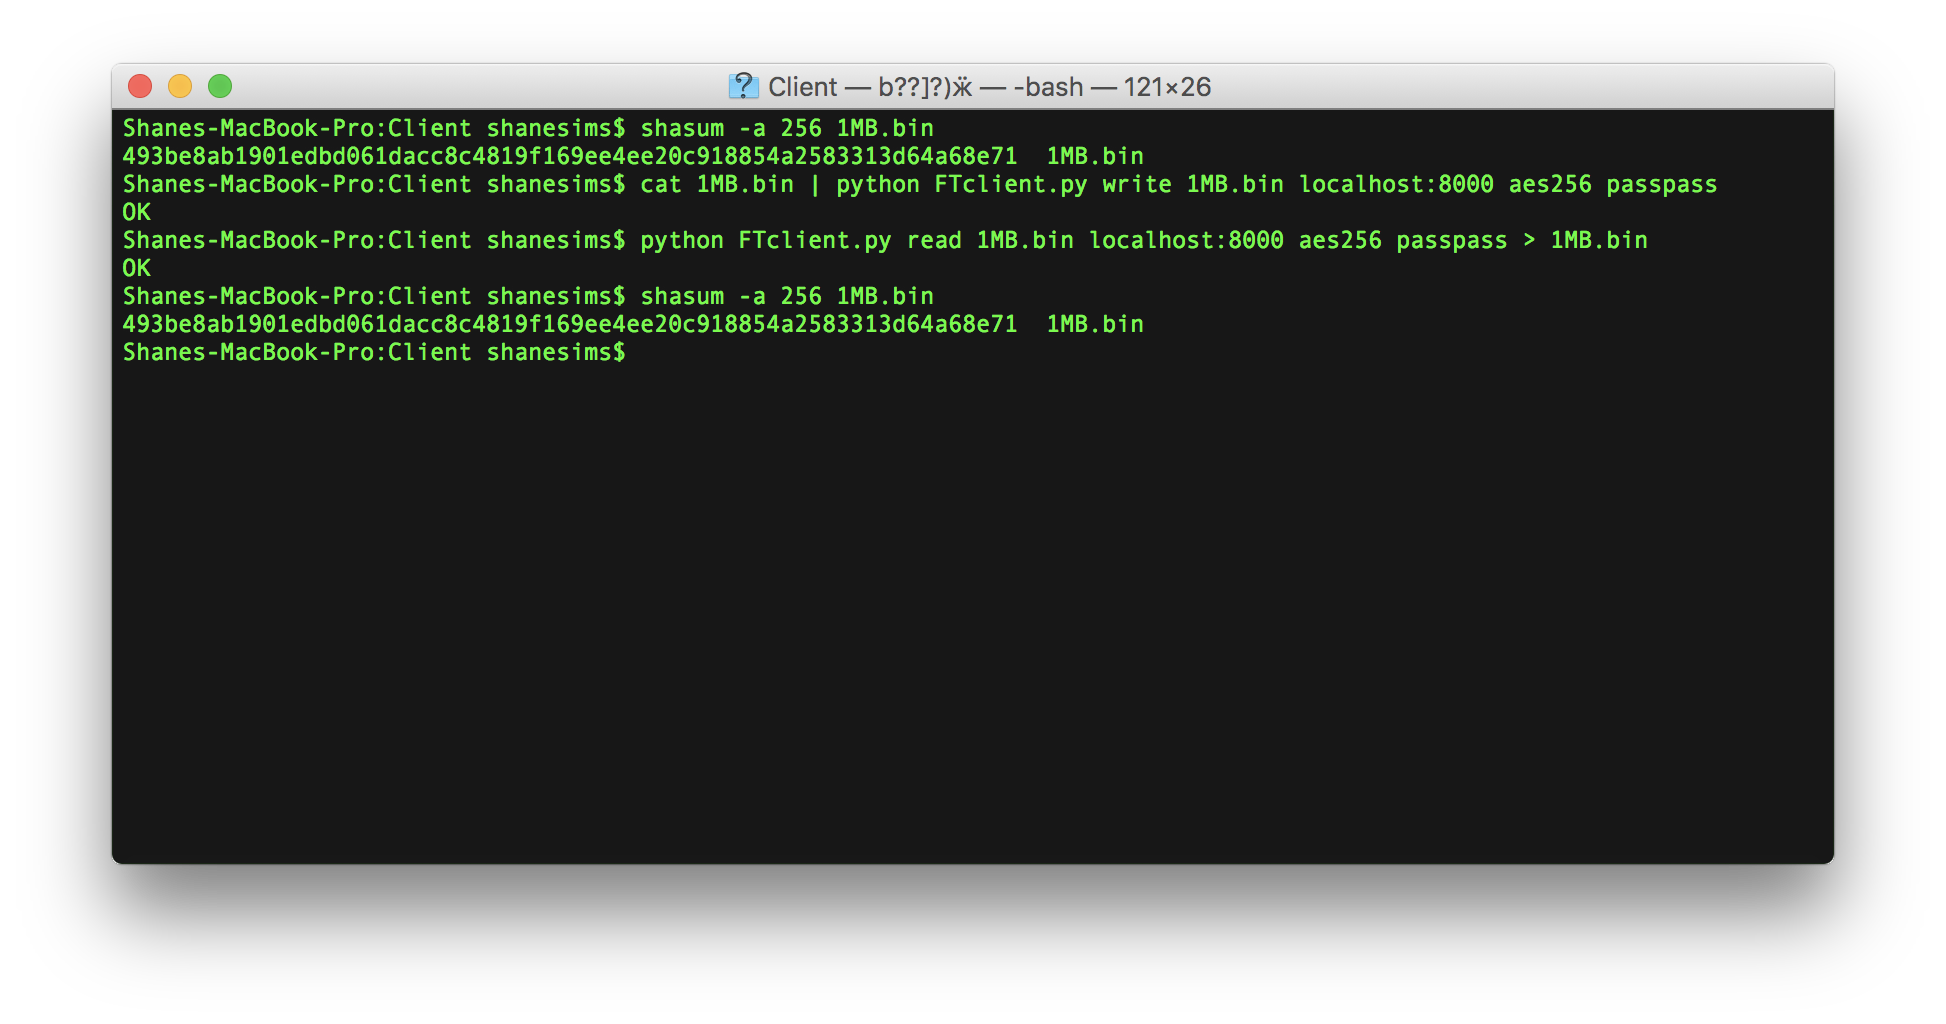
\includegraphics[scale=0.5, trim={0cm 0cm 0cm 0cm}, clip]{test}
	\caption{Test for correctness}
	\end{figure}

\section*{Communication Protocol}
\subsection*{\texttt{write} command}
\begin{center}
\begin{tabular}{ |c|c|c| } 
 \hline
 ~& Client & Server\\
 \hline\hline
 1. & send cipher,nonce1 & ~\\
 \hline
 2. & ~& send challenge nonce2 \\
 \hline
 3. & send sha256(key|nonce2) & ~ \\
 \hline
 4. & ~& send ACK\\
 \hline
 5. & send \texttt{write} & ~ \\ 
 \hline
 6. & ~ & send ACK\\ 
 \hline
 7. & send \texttt{fileName} & ~ \\ 
 \hline
 8. & ~ & echo \texttt{fileName}\\
 \hline
 9. & encrypt 1024 byte blocks and \texttt{send} & ~\\
 \hline
 10. & ~& \texttt{receive} and decrypt blocks\\
 \hline
 11. &\texttt{send} EOF &~\\
 \hline
 12. & ~& \texttt{send} status/result flag\\
 \hline
 13. & \texttt{print} status & ~\\
 \hline
\end{tabular}
\end{center}

\subsection*{\texttt{read} command}
\begin{center}
\begin{tabular}{ |c|c|c| } 
 \hline
 ~& Client & Server\\
 \hline\hline
 1. & send cipher,nonce1 & ~\\
 \hline
 2. & ~& send challenge nonce2 \\
 \hline
 3. & send sha256(key|nonce2) & ~ \\
 \hline
 4. & ~& send ACK\\
 \hline
 5. & \texttt{send} \texttt{read} & ~ \\ 
 \hline
 6. & ~ & \texttt{send} {ACK} \\ 
 \hline
 7. & \texttt{send} file name & ~ \\ 
 \hline
 8. & ~ & \texttt{send} file size\\
 \hline
 9. & ~& encrypt 1024 byte blocks and \texttt{send}\\
 \hline
 10. & \texttt{receive} and decrypt blocks &~\\
 \hline
 11. & \texttt{send} status/result flag &~\\
 \hline
 12. & \texttt{print} status & ~\\
 \hline
\end{tabular}
\end{center}


\section*{Timing Tests}

	\begin{figure}[H]
	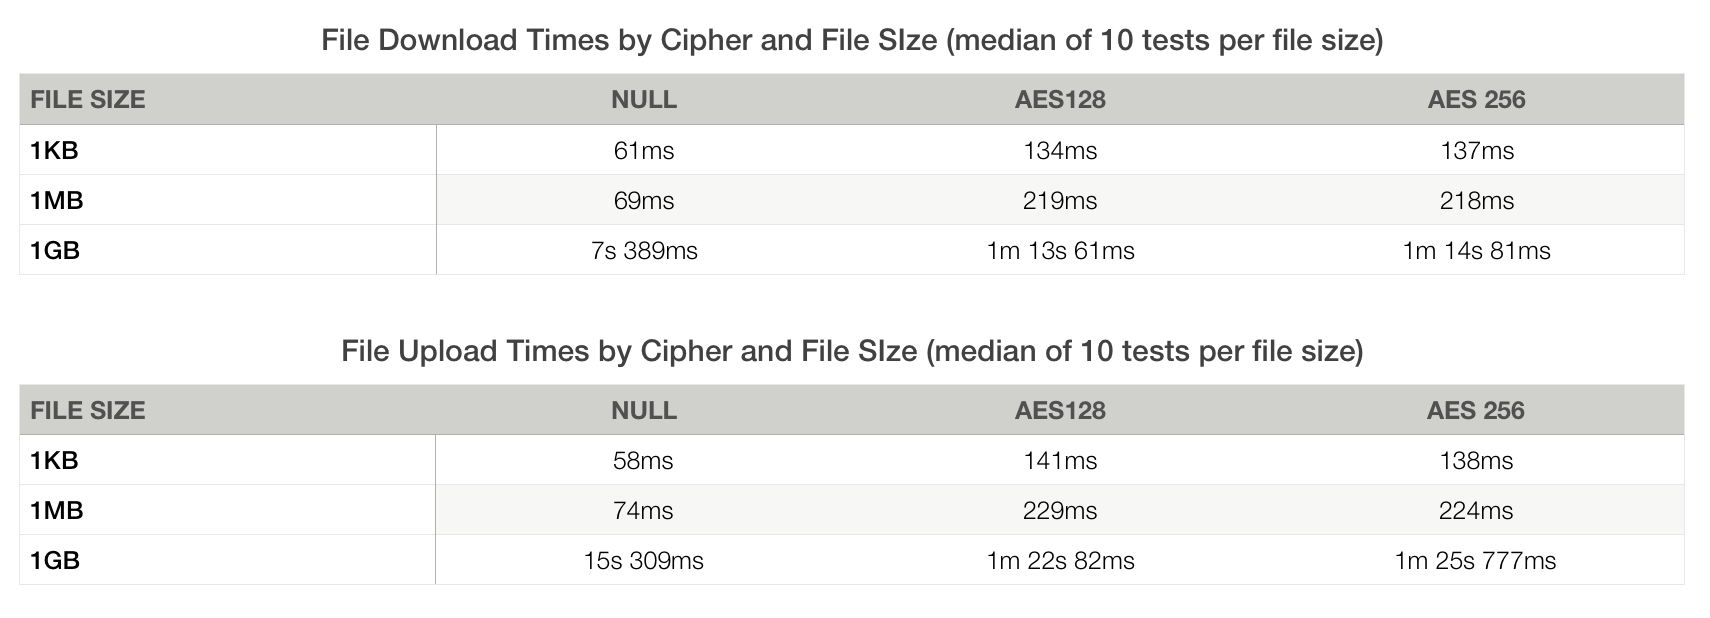
\includegraphics[scale=0.5, trim={0cm 0cm 0cm 0cm}, clip]{time_tab}
	\caption{}
	\end{figure}

Summary of Results:\newline

\begin{itemize}
	\item Download times: From the figure above, it appears that there is a negligible difference in the download times the two AES ciphers used. It might have been expected that the time to download the 1GB file would have resulted in a pronounced difference between the two AES ciphers, but this was not the case. Somewhat surprisingly, within a given AES cipher there the download times for the 1MB file was about twice that of the 1KB file, despite being nearly ten times the size.  As was to be expected, the download speed of when using the null cipher was much faster than using the either of the AES ciphers, in all cases of file size. 
	\item Upload times: From the figure above, it can be seen that the results of the time tests for uploading are very similar to those for downloading, for all ciphers and file sizes. The only noteworthy comment that can be made is that on average the upload times were slightly slower than those for downloads.
\end{itemize}


\end{document}

